\documentclass{article}

\usepackage[dblblindworkshop, final]{neurips2025}
% Note. For the workshop paper template, both \title{} and \workshoptitle{} are required, with the former indicating the paper title shown in the title and the latter indicating the workshop title displayed in the footnote.
% For workshops (5., 6.), the authors should add the name of the workshop, "\workshoptitle" command is used to set the workshop title.
% \workshoptitle{WORKSHOP TITLE}

% "preprint" option is used for arXiv or other preprint submissions
 % \usepackage[preprint]{neurips_2025}

% to avoid loading the natbib package, add option nonatbib:
%    \usepackage[nonatbib]{neurips_2025}

\usepackage[utf8]{inputenc} % allow utf-8 input
\usepackage[T1]{fontenc}    % use 8-bit T1 fonts
\usepackage{hyperref}       % hyperlinks
\usepackage{url}            % simple URL typesetting
\usepackage{minted}
% \usepackage[finalizecache,cachedir=_minted-neurips2025]{minted}
% \usepackage{listings}
\usepackage{booktabs}       % professional-quality tables
\usepackage{amsfonts}       % blackboard math symbols
\usepackage{nicefrac}       % compact symbols for 1/2, etc.
\usepackage{microtype}      % microtypography
\usepackage{xcolor}         % colors
\usepackage{graphicx}
\usepackage{pifont}     % For the check and cross marks
\usepackage[dvipsnames]{xcolor} % For custom colors
\usepackage{graphicx}
\usepackage{multirow}

\newcommand{\cmark}{\ding{51}}%
\newcommand{\xmark}{\ding{55}}%
\newcommand{\yes}{\textcolor{OliveGreen}{\cmark}}
\newcommand{\no}{\textcolor{BrickRed}{\xmark}}


% Note. For the workshop paper template, both \title{} and \workshoptitle{} are required, with the former indicating the paper title shown in the title and the latter indicating the workshop title displayed in the footnote. 
\title{\textsc{Quran-MD}: A Fine-Grained Multilingual Multimodal Dataset of the Quran}




% The \author macro works with any number of authors. There are two commands
% used to separate the names and addresses of multiple authors: \And and \AND.
%
% Using \And between authors leaves it to LaTeX to determine where to break the
% lines. Using \AND forces a line break at that point. So, if LaTeX puts 3 of 4
% authors names on the first line, and the last on the second line, try using
% \AND instead of \And before the third author name.


\author{%
  Muhammad Umar Salman \\
  MBZUAI\\
  Abu Dhabi, UAE\\
  \texttt{umar.salman@mbzuai.ac.ae} \\
  % examples of more authors
  \And
  Mohammad Areeb Qazi \\
  MBZUAI\\
  Abu Dhabi, UAE\\
  \texttt{mohammad.qazi@mbzuai.ac.ae} \\
   \And
  Mohammed Talha Alam \\
  MBZUAI\\
  Abu Dhabi, UAE\\
  \texttt{mohammed.alam@mbzuai.ac.ae} \\
  % Coauthor \\
  % Affiliation \\
  % Address \\
  % \texttt{email} \\
  % \AND
  % Coauthor \\
  % Affiliation \\
  % Address \\
  % \texttt{email} \\
  % \And
  % Coauthor \\
  % Affiliation \\
  % Address \\
  % \texttt{email} \\
  % \And
  % Coauthor \\
  % Affiliation \\
  % Address \\
  % \texttt{email} \\
}


\begin{document}


\maketitle


\begin{abstract}
  We present \textsc{Quran-MD}, a comprehensive multimodal dataset of the Qur’an that integrates textual, linguistic, and audio dimensions at the verse and word levels. For each verse (ayah), the dataset provides its original Arabic text, English translation, and phonetic transliteration. To capture the rich oral tradition of Qur’anic recitation, we include verse-level audio from 32 distinct reciters, reflecting diverse recitation styles and dialectical nuances. At the word level, each token is paired with its corresponding Arabic script, English translation, transliteration, and an aligned audio recording, allowing fine-grained analysis of pronunciation, phonology, and semantic context. This dataset supports various applications, including natural language processing, speech recognition, text-to-speech synthesis, linguistic analysis, and digital Islamic studies. Bridging text and audio modalities across multiple reciters, this dataset provides a unique resource to advance computational approaches to Qur’anic recitation and study. Beyond enabling tasks such as ASR, tajweed detection, and Qur’anic TTS, it lays the foundation for multimodal embeddings, semantic retrieval, style transfer, and personalized tutoring systems that can support both research and community applications. The dataset is available at \url{https://huggingface.co/datasets/Buraaq/quran-audio-text-dataset}

\end{abstract}

\section{Introduction}
\label{sec:intro}

The Qur’an, the holy book of Islam, occupies a central role in the spiritual, intellectual, and cultural lives of nearly two billion Muslims worldwide. Revealed in Classical Arabic (Fusha), it is not only revered as sacred scripture but also preserved through its oral tradition of recitation. Mastery of recitation is guided by tajweed which is a set of phonological and prosodic rules that ensure the Qur’an is read with precision, beauty, and correctness. For Muslims, engaging with the Qur’an involves more than simply reading the text but is an act of devotion that requires both accurate pronunciation and a deep understanding of its meaning.

Despite its origins in Arabic, the Qur’an is recited and studied across every corner of the globe, including by millions of non-Arabic speakers from diverse linguistic and cultural backgrounds. This global engagement highlights the challenges faced by learners who must navigate not only the Arabic script but also its sounds, phonology, and interpretive meanings. While Islamic scholars, including Ulama (religious scholars), Fuqaha (jurists), and researchers, have made significant contributions to Qur’anic studies, the integration of modern computational approaches, particularly artificial intelligence, remains very limited compared to the rapid advances in AI. AI has the potential to illuminate linguistic patterns, aid recitation training, and support both Arabic and non-Arabic learners in mastering tajweed and understanding the Qur’an’s message.

Existing resources, however, often fall short of capturing the Qur’an’s full multimodal nature. Some datasets provide the Arabic text alone, others include translations or transliterations, and a few extend to audio recordings at either the verse or word level. Rarely are these modalities combined in a way that allows fine-grained analysis of both the written and spoken Qur’an. This fragmentation restricts their utility for advancing AI-driven research in areas such as natural language processing, speech recognition, and text-to-speech synthesis. Table \ref{tab:comparison_final} summarizes key features of prior Qur’anic datasets, where \textsc{Qur’an-MD} offers the most comprehensive multimodal coverage.

In this work, we curate and harmonize resources from three data sources to construct \textsc{Qur’an-MD}, a comprehensive multimodal dataset of the Qur’an. Our dataset unifies Arabic text, English translation, and phonetic transliteration at both the verse and word levels, while pairing each word with an aligned audio recording of its pronunciation. We provide high-quality recitations from 30 distinct reciters at the verse level, representing diverse styles and dialectical nuances (see Table \ref{tab:dataset_stats} in the Appendix). Through careful validation and consistency checks, we ensure the reliability of the textual and audio components. By making this dataset available on Hugging Face, we aim to provide scholars, linguists, and AI researchers with a standardized resource that bridges textual, phonological, and semantic dimensions. This contribution supports the study of Qur’anic language and recitation traditions. It enables and promotes future work in cutting-edge computational applications at the intersection of speech, language, and Quranic studies. 
\section{Related Work}

There has been growing interest in developing resources for Qur’anic text and recitation, yet existing efforts typically focus on either textual analysis or audio recordings, rather than providing a fully integrated multimodal resource. Early structured corpora, such as the \emph{Quranic Arabic Corpus} \cite{dukhovny2009qac}, provide full text with detailed morphological and syntactic annotations, supporting parsing, part-of-speech tagging, and grammatical analysis. More recent contributions, including the \emph{MASAQ corpus} \cite{sawalha2024masaq} and the corpus introduced by \cite{nashir2025quranic}, expand these annotations and incorporate orthographic variants (Uthmani and Imlaai scripts), Buckwalter and phonetic transliterations, as well as English translations at the verse level. Similarly, the \emph{Tanzil project} \cite{tanzil2008} offers the Qur’an aligned with translations in more than 40 languages, supporting multilingual NLP research, though without detailed linguistic or recitational information.

\begin{table*}[t]
\centering
\caption{Feature comparison across prominent Quranic datasets. The proposed \textsc{Qur’an-MD} is the first to holistically integrate all listed modalities across multiple reciters at both verse and word levels, filling a critical gap in the available resources.}
\label{tab:comparison_final}
\resizebox{0.9\textwidth}{!}{%
\begin{tabular}{@{}lccccc@{}}
\toprule
 & \multicolumn{5}{c}{\textbf{Dataset}} \\
\cmidrule(l){2-6}
\textbf{Feature} & \begin{tabular}[c]{@{}c@{}}Quranic Arabic \\ Corpus \cite{dukhovny2009qac}\end{tabular} & \begin{tabular}[c]{@{}c@{}}Tanzil \\ Project \cite{tanzil2008}\end{tabular} & Tarteel \cite{khan2021tarteel} & QDAT \cite{qdat2021} & \begin{tabular}[c]{@{}c@{}}\textbf{\textsc{Qur’an-MD}} \\ \textbf{(Ours)}\end{tabular} \\ 
\midrule
Text (Arabic) & \yes & \yes & \yes & \yes & \yes \\
Morpho-syntactic Data & \yes & \no & \no & \no & \yes \\
Multi-Language Translation & \no & \yes & \no & \no & \yes \\
Word-level Audio & \no & \no & \no & \yes & \yes \\
Verse-level Audio & \no & \no & \yes & \yes & \yes \\
Multiple Reciters & \no & \no & \yes & \no & \yes \\ 
\bottomrule
\end{tabular}%
}
\end{table*}


Parallel to these textual resources, several initiatives have sought to capture Qur’anic recitation across multiple readers. Large-scale audio collections, such as \emph{Tarteel AI EveryAyah}\cite{khan2021tarteel} and the \emph{Quran-Recitations Dataset} \cite{quran_recitations_hf_dataset}, provide verse-level recordings across numerous reciters, while the \emph{Quranic Audio Dataset} \cite{quran_audio_dataset2024} and \emph{RetaSy} \cite{salameh2024retasy} focus on non-native reciters with labeled correctness annotations. The \emph{OpenSLR Quran Speech-to-Text corpus} \cite{openslr132} offers complete verse coverage for multiple reciters, and smaller targeted collections, such as \emph{QDAT} \cite{osman2021qdat} and its extensions \cite{eval_pronunciation_tajweed2025}, provide labeled data for Tajweed error detection using deep neural models. Recent Kaggle contributions, including the \emph{Quran Ayat Speech-to-Text} dataset \cite{bigguyubuntu2023ayat}, \emph{Quran Reciters dataset} \cite{omartariq2025}, \emph{Quran.com Audio dataset} \cite{abdo3id2022qurancom}, \emph{Quran Recitations for Audio Classification dataset} \cite{alrajeh2021recitations}, and the \emph{Comprehensive Quranic Dataset v1 (CQDV1)} \cite{cqdv12024}, offer large-scale verse-level audio recordings from dozens of reciters, but generally provide only Arabic text and audio without consistent transliteration or translation.

Taken together, these resources demonstrate substantial progress in both linguistic annotation and audio collection, yet they remain fragmented: either focusing on text or audio, verse- or word-level data. None combine verse and word-level text, transliteration, English translation, and audio across multiple reciters with consistent cross-modal alignment. \textsc{Qur’an-MD} addresses these gaps by integrating verse and word-level text, English translation, transliteration, word-level audio, and verse audio from 30 reciters, providing a unified multimodal resource that supports research across natural language processing, speech technologies, linguistic analysis, and digital Islamic studies.
 
\section{Dataset (\textsc{Qur’an-MD})}
\label{sec:dataset-preparation}

The dataset was constructed by aggregating and harmonizing three publicly available sources of Qur’anic data: (1) a Kaggle dataset of verse-level speech-to-text recordings by 30 reciters \cite{quran_ayat_speech_kaggle}, (2) the \texttt{quranwbw} repository containing aligned word-by-word Arabic text, English translations, and transliterations \cite{quranwbw_repo}, and (3) the Internet Archive collection of word-by-word Qur’an audio recordings \cite{quran_wordbyword_archive}. To unify these heterogeneous resources, we designed a hierarchical JSON template. At the top level, each \texttt{surah} (chapter) is represented by its numerical index (e.g., \texttt{"112"} for the 114 surah's) and annotated with its Arabic name, English translation, transliteration, and total verse count. Each surah contains a nested set of \texttt{verses} (ayahs), where each verse entry includes the Arabic text, its English translation, phonetic transliteration, paths to reciter-specific verse-level audio, and a list of word-level objects. Word objects store the word Arabic script, English translation, transliteration, and the corresponding aligned audio file. This structure allows seamless integration of textual, transliterated, and auditory modalities across both verse- and word-level granularities.  

The preparation pipeline proceeded in four main steps. First, surah-level metadata (surah number, names, and verse counts) was populated into the template. Second, from the Kaggle dataset, verse-level recitations by 30 reciters were aligned with their corresponding verse texts and added under the \texttt{audio\_ayah\_path} field. Third, word-level Arabic text, translations, and transliterations from the \texttt{quranwbw} repository were inserted into the template. Fourth, word-level audio files from the Internet Archive collection were matched to individual tokens and linked under the \texttt{audio\_word\_path} field. After populating all layers, automated validation scripts were applied to ensure correctness, checking that every word and verse was paired with its corresponding audio, and identifying and correcting missing or misaligned entries. This pipeline resulted in a complete, consistent, and multimodal representation of the Qur’an, ready for release as a standardized dataset.

\textbf{Dataset Format}: The dataset is organized in a hierarchical JSON structure, where each surah (chapter) of the Qur’an is represented as a nested object. This design ensures that verse-level and word-level information is consistently accessible and easily parsable for downstream applications. An example of Surah 112 (\textit{Al-Ikhlas}) is shown in Figure \ref{fig:example} (Appendix), highlighting metadata and audio/text linkage. This structure enables researchers to work seamlessly at both the verse level (for example, analyzing prosody between reciters) and the word level (for example, studying phoneme-grapheme alignment).

\begin{figure}[htp]
    \centering
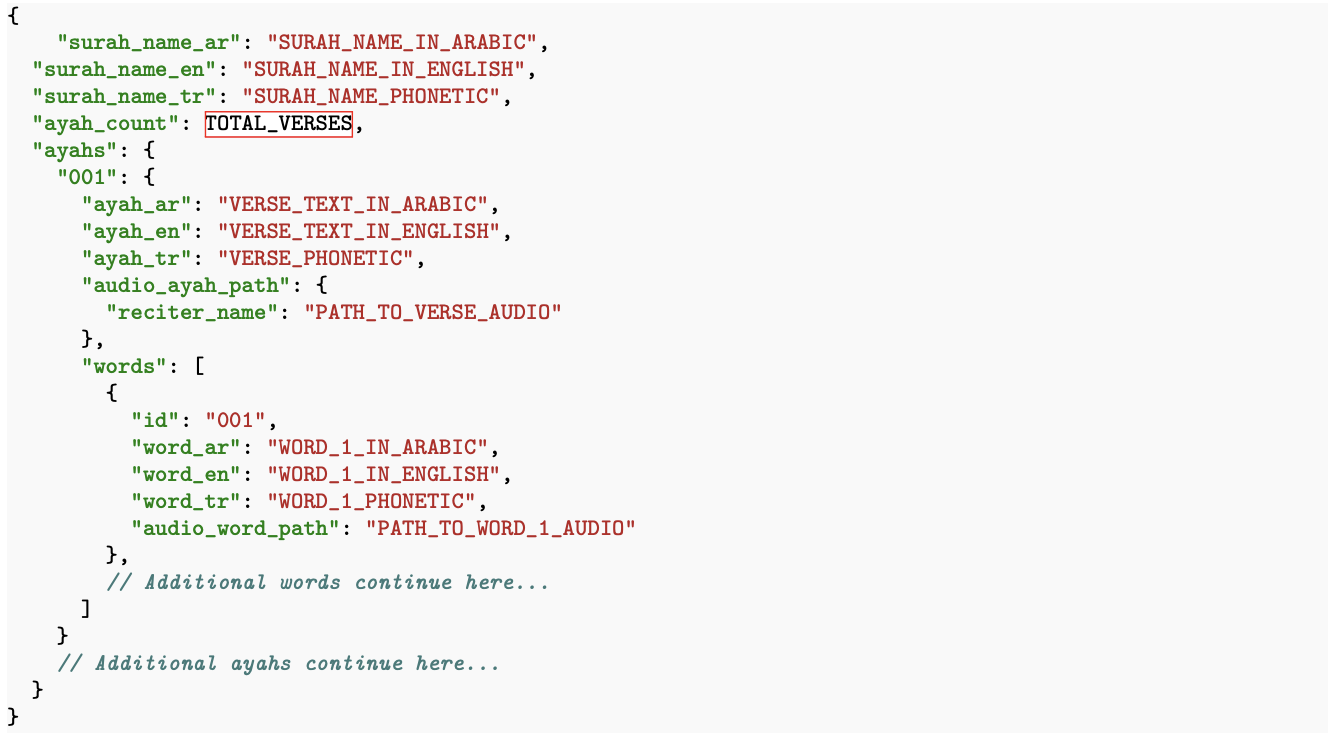
\includegraphics[width=\textwidth]{figures/fing.png} % Adjust width as needed
    % \caption{Example of format of Surah 112 (Al-Ikhlas) in the Dataset.}
    \label{fig:fing}
\end{figure}

% \begin{minted}[fontsize=\scriptsize, breaklines, bgcolor=lightgray!10]{json}
% { 
%     "surah_name_ar": "SURAH_NAME_IN_ARABIC",
%   "surah_name_en": "SURAH_NAME_IN_ENGLISH",
%   "surah_name_tr": "SURAH_NAME_PHONETIC",
%   "ayah_count": TOTAL_VERSES,
%   "ayahs": {
%     "001": {
%       "ayah_ar": "VERSE_TEXT_IN_ARABIC",
%       "ayah_en": "VERSE_TEXT_IN_ENGLISH",
%       "ayah_tr": "VERSE_PHONETIC",
%       "audio_ayah_path": {
%         "reciter_name": "PATH_TO_VERSE_AUDIO"
%       },
%       "words": [
%         {
%           "id": "001",
%           "word_ar": "WORD_1_IN_ARABIC",
%           "word_en": "WORD_1_IN_ENGLISH",
%           "word_tr": "WORD_1_PHONETIC",
%           "audio_word_path": "PATH_TO_WORD_1_AUDIO"
%         },
%         // Additional words continue here...
%       ]
%     }
%     // Additional ayahs continue here...
%   }
% }
% \end{minted}
% Research directions enabled by your multimodal Qur’an dataset

% I divide them into: (A) Speech-only, (B) Text-only / NLP, (C) Speech + Text (multimodal), and (D) Tools & Applications. For each I include: what to build, why your dataset helps, methods/approaches, evaluation ideas, and main challenges.

% A — Speech-only (audio-focused)
% A1 — Qur’anic ASR (verse- and word-level)

% What: Train automatic speech recognition systems specialized for Qur’anic recitation (word/verse transcription, segmentation).
% Why dataset helps: You have aligned word-level audio + text and many reciters → enables supervised ASR with variation across voices and recitation styles.
% Approach: End-to-end ASR (Conformer / Wav2Vec2 / Whisper-style fine-tuning) with language model boosting for Classical Arabic text; optionally adapt a grapheme-to-phoneme module for tajweed-influenced pronunciations. Use per-word audio for fine-grained segmentation models.
% Eval: Word error rate (WER) on verse and on token-level, boundary detection metrics (F1) for segmentation, per-reciter and cross-reciter WER.
% Challenges: Classical (Fusha) Qur’anic orthography differs from modern corpora; long melodic stretching (madd), pauses, and Quranic tajweed rules create unusual acoustic patterns that need modeling. See prior ASR overviews and datasets. 
% ResearchGate

% A2 — Automatic detection/classification of Tajweed rules (mispronunciation tagging)

% What: Detect occurrences of tajweed phenomena (e.g., madd, ghunnah, idgham, ikhfa, tafkheem/tarqeeq) or identify mistakes in learners’ recitations.
% Why dataset helps: Word-level audio aligned with canonical text allows supervised labels (you could annotate examples or derive weak labels from expert recitations). Existing smaller datasets (e.g., QDAT) target this task but are limited in size/diversity — your dataset can scale this. 
% ResearchGate
% +1

% Approach: Frame-level or segment-level classifiers (CNN/transformer on spectrograms; sequence labeling with CTC or token classification); combine acoustic features with phonetic/linguistic features (G2P outputs, rule-based signals). Use multi-task learning to jointly detect multiple tajweed phenomena.
% Eval: Precision/recall/F1 per rule; accuracy of error detection for beginner vs expert recitations; human expert validation.

% A3 — Reciter identification and voice profiling

% What: Given a verse or segment, identify the reciter (voice recognition) or cluster reciters by style/dialect.
% Why dataset helps: 32 reciters × consistent verse coverage → ideal for speaker ID, voice-style analysis, and voice-clustering research.
% Approach: Speaker embeddings (x-vectors, ECAPA-TDNN), contrastive learning across verses to capture style-invariant features; investigate style vs content disentanglement.
% Eval: Top-1/top-5 accuracy for reciter ID; clustering metrics (ARI, NMI) for style groupings; cross-reciter generalization tests.
% Challenges: Reciters sometimes change style or tempo; dataset does allow large-scale study though. Several recent papers use similar reciter datasets for speaker/classification tasks. 
% Natural Science Publishing

% A4 — Prosody & melodic analysis (intonation, madd duration modeling)

% What: Measure and model prosodic patterns, stretch durations, pause insertion patterns, and melodic contours of recitation styles.
% Why dataset helps: Multiple reciters reciting same verses lets you analyze prosody independent of lexical content.
% Approach: Extract F0, duration, intensity, align to tokens; use sequence models to predict expected madd lengths, or to synthesize recitation prosody for TTS.
% Eval: Correlation between predicted and real durations/F0; listening tests for synthesized prosody.

% B — Text-only (NLP / classical Arabic)
% B1 — Token-level morphological analysis & diacritization for Qur’anic Arabic

% What: Automatic diacritization (short vowels/harakat) and morphological parsing specialized for Classical Qur’anic Arabic.
% Why dataset helps: Word-level tokens with transliteration and aligned audio can supervise diacritization and pronunciation-to-text mapping.
% Approach: Sequence-to-sequence or transformer diacritization models; multimodal input (audio + orthography) to improve disambiguation.
% Eval: Diacritization error rate, morphological tagging accuracy.

% B2 — Semantic retrieval, question answering, and RAG (Qur’anic knowledge retrieval)

% What: Build retrieval-augmented systems to answer queries using Qur’anic text + translations + tafsir (if available).
% Why dataset helps: Fine-grained word-level translations + verse-level context support better chunking, retrieval and grounding for LLMs.
% Approach: Create embeddings (text-only or multimodal) per verse/word for vector search; fine-tune LLM or use RAG pipelines for QA grounded in the Qur’an.
% Eval: Retrieval metrics (recall@k), QA accuracy vs human-annotated answers, faithfulness metrics.

% B3 — Alignment of translation and transliteration to source tokens

% What: Create reliable mappings between Arabic tokens and English translations at word-level (not trivial: translation is often non-literal or many-to-one).
% Why dataset helps: You already have per-word English translations and transliterations that can be used to train alignment models or to produce better bilingual lexicons.
% Approach: Use attention-based alignment models or alignment via forced alignment (multimodal cues). Train word-level bilingual embeddings.
% Eval: Alignment precision/recall vs human alignments.

% C — Multimodal (speech + text together) — where your dataset excels
% C1 — Word-level forced-alignment and phoneme-level segmentation

% What: Accurate alignment between Arabic orthography and audio at word/phoneme level (time-stamps for each token).
% Why dataset helps: You have word-level audio files which can bootstrap or supervise alignment; many prior works lack this fine-grain mapping at scale.
% Approach: Use Kaldi / Montreal Forced Aligner or neural forced alignment with CTC-based models; train acoustic models using the canonical tokens as transcripts.
% Eval: Boundary error (seconds), percent tokens aligned correctly. This alignment is foundational for other downstream tasks (pronunciation modeling, TTS unit extraction).

% C2 — Pronunciation tutoring & automated feedback for learners

% What: Systems that listen to a learner recite, detect tajweed issues, and provide targeted, explainable feedback with audio examples.
% Why dataset helps: Canonical recitations from 32 expert reciters act as high-quality references; word-level audio enables precise corrective examples.
% Approach: Combine ASR + tajweed-classifier + sequence alignment to highlight mismatches; create explainable feedback modules with synthetic examples (show correct audio, visual articulatory cues).
% Eval: Expert-rated improvement in learner recitation; detection precision/recall for learner mistakes (user studies).

% C3 — Qur’an TTS that respects tajweed and recitation styles

% What: A TTS system that synthesizes Qur’anic recitation obeying tajweed rules and optionally mimics specific reciters’ melodic style.
% Why dataset helps: Parallel verse coverage for 32 reciters allows multi-speaker TTS training and style-transfer (voice cloning) while word-level audio helps unit selection or neural vocoder conditioning on pronunciation/pronunciation duration (madd).
% Approach: Modern neural TTS (FastSpeech2 + HiFi-GAN) with style embeddings, or fine-tune multi-speaker Tacotron/Glow-TTS; include tajweed-informed linguistic front-end (G2P + prosody markers). Consider neural prosody modeling conditioned on tajweed labels. Prior TTS/Quran attempts show feasibility but often with limited corpora. 
% Ijassat
% +1

% Eval: MOS for naturalness and tajweed correctness, expert evaluation for adherence to recitation norms.

% C4 — Cross-reciter style transfer and voice conversion with tajweed preservation

% What: Convert a recitation from one reciter to sound like another while preserving tajweed-correct pronunciation and prosody.
% Why dataset helps: Same textual content across many reciters gives parallel (or near-parallel) training data; word-level audio helps aligning units for conversion.
% Approach: Voice conversion methods (GAN/flow-based or neural-adaptive). Add constraints to preserve phonetic realization consistent with tajweed.
% Eval: Speaker similarity (speaker verification), intelligibility, and expert-rated tajweed adherence.

% C5 — Multimodal embeddings & downstream tasks (classification, retrieval)

% What: Learn joint audio-text embeddings for semantically-aware indexing (e.g., search by meaning + recitation style).
% Why dataset helps: Paired audio and text across many reciters allows multimodal representation learning that can capture both meaning and acoustic style.
% Approach: Contrastive multimodal pretraining (e.g., CLIP-style for audio-text), then use embeddings for retrieval, clustering, or transfer learning.
% Eval: Retrieval metrics, clustering coherence, downstream task gains (e.g., better ASR under low-resource conditions using multimodal pretraining).

% D — Applications, tooling & community resources
% D1 — Evaluation suites & benchmarks

% Create standardized test splits (per-surah, per-reciter) and tajweed-annotated test sets for community benchmarking (ASR, tajweed detection, TTS). Several recent works highlight the need for shared benchmarks. 
% arXiv

% D2 — Data augmentation and synthetic learner errors

% Generate controlled mispronunciations and synthetic learner recitations for robust training of error-detection and tutoring models. Papers synthesize errors for controlled evaluation in similar domains. 
% arXiv

% D3 — Tools for scholars: aligned corpora for linguistic / phonological research

% Offer easy-to-use APIs and visualizers (word audio players, aligned waveform + transcript viewers) to support humanities researchers and teachers.

% Suggested baseline experiments (practical starting points)

% ASR baseline — Fine-tune a pre-trained wav2vec2 model on your verse-level data; report WER per-reciter and averaged. Compare training on verse-level transcripts vs using word-level audio as additional fine-tuning data.

% Tajweed classifier baseline — Use QDAT-style labels (or create new labels) to train a CNN+LSTM classifier on spectrograms to identify a set of tajweed rules. Evaluate using F1. (QDAT and other papers provide a reference setup). 
% ResearchGate
% +1

% Forced-aligner baseline — Use Montreal Forced Aligner with an Arabic acoustic model trained on your word-audio to produce phoneme/time alignments; evaluate boundary error against manual checks.

% Multi-speaker TTS baseline — Train a multispeaker FastSpeech2 conditioned on reciter IDs and tajweed prosody tags; evaluate MOS + tajweed expert score.

% Evaluation metrics and human evaluation

% Automatic: WER/CER, precision/recall/F1 for tajweed classes, boundary error (ms), MOS (naturalness), speaker-ID accuracy, embedding retrieval metrics (recall@k).

% Human/Expert: Expert tajweed adherence score, MOS with domain experts, pedagogical usefulness in small user studies (does feedback help learners improve?). Prior work emphasizes expert validation for tajweed tasks. 
% ResearchGate
% +1

% Main challenges & gaps (research opportunities)

% Classical Qur’anic text vs Modern Arabic: Models pre-trained on modern corpora may mis-handle classical orthography, archaisms, and specific punctuation/pauses; domain-adaptation is needed.

% Tajweed-sensitive modeling: Tajweed rules create acoustic phenomena (madd, nasalization) that standard speech models don’t normally account for — specialized phonetic modeling and G2P with tajweed features are needed. 
% Ijassat

% Evaluation standardization: Lack of widely accepted benchmark splits and tajweed annotation conventions hinders cross-paper comparability — your dataset can host benchmark suites. 
% arXiv

% Cultural/ethical considerations: Recitation is a religious practice; synthetic recitations or voice cloning must be handled respectfully, with opt-in consent or clear purpose statements for the community.

\section{Future Work}

\textsc{Qur’an-MD} opens multiple avenues for future research at the intersection of speech processing, natural language processing, and digital Islamic studies. We outline three directions: (A) Speech-only tasks, (B) Multimodal approaches integrating speech and text, and (C) Tools and applications that can support both research and community engagement.  

\textbf{Speech-only Research}: A major direction lies in automatic speech recognition (ASR) for Qur’anic recitation, both at the verse and word level. The audio and verse-level transcripts aligned in the dataset with 30 reciters provide a unique testbed to develop end-to-end ASR models adapted to classical Arabic with the unique prosody and melodic contours in recitations. Evaluations can measure word error rate and segmentation accuracy across reciters, while challenges include modeling tajweed-driven prosody (madd, pauses, emphatics) and script-pronunciation mismatches.  

\textbf{Multimodal Speech-Text Research}: The full potential emerges when the modalities are combined. The dataset can drive progress in forced alignment and phoneme-level segmentation, producing high-quality timestamps for words and phonemes that benefit pronunciation modeling. It enables pronunciation tutoring systems tailored to Qur’anic recitation, which automatically detect tajweed issues and mispronounced words, providing corrective audio feedback and guidance on proper melodic and rhythmic patterns.

Another promising direction is Qur’anic TTS that respects tajweed rules and recitation styles. Leveraging parallel recordings from 32 reciters, the dataset enables the development of personalized TTS systems that provide corrective feedback for tajweed and Qur’anic melody in a user’s own voice, facilitating accurate imitation and learning. In addition, style transfer approaches can allow users to reproduce the prosody and melodic patterns of renowned reciters while preserving tajweed correctness, supporting both educational applications and expressive recitation synthesis. 

\textbf{Tools, Applications, and Community Resources:} \textsc{Qur’an-MD} also enables the development of advanced tools and applications that bridge research and community engagement. Multimodal embeddings of Qur’anic text and audio can support semantic retrieval of specific verses, style-aware search, and clustering of reciters, while facilitating the creation of robust tutoring systems for pronunciation and tajweed. Beyond machine learning applications, the dataset can be integrated into retrieval platforms, APIs, and interactive visualization tools for scholars, educators, and students, providing aligned verse- and word-level corpora that support linguistic, phonological, and prosodical research. Such resources can foster broader accessibility and engagement with the Qur'an and its studies.


% \textbf{Text-only / NLP Research}: On the text side, word-level annotations facilitate \emph{diacritization and morphological analysis} for classical Qur’anic Arabic, a long-standing challenge due to complex orthography. Incorporating aligned transliterations and pronunciations may further reduce diacritization errors. Another direction is \emph{semantic retrieval and question answering}, where embedded in aligned Arabic--English pairs can improve retrieval-augmented generation for Qur’anic queries. The dataset also enables research on \emph{alignment of translations and transliterations}, resulting in more accurate bilingual lexicons and improving cross-lingual applications in Islamic studies.  
\section{Conclusion}
\label{sec:conclusion}

We curated \textsc{Qur’an-MD}, a comprehensive multimodal dataset of the Qur’an from three different sources that integrates textual and audio information with linguistic annotations at the verse- and word-level, encompassing 30 distinct reciters to capture the rich diversity of Qur’anic recitation. By aligning Arabic text, English translations, phonetic transliterations, and fine-grained audio recordings at both verse- and word-levels, the dataset enables a wide range of research applications, including automatic speech recognition, tajweed detection, pronunciation tutoring, personalized Qur’anic TTS, style transfer, and prosody modeling. Furthermore, it supports the development of multimodal embeddings for semantic retrieval, style-aware search, and reciter clustering, as well as interactive tools for scholars, educators, and learners. This resource bridges text and audio modalities at scale, providing a unique platform to advance computational modeling and applications in Qur’anic research.
 
\newpage
\section{Appendix}  

Beyond ASR, the dataset can enable automatic tajweed detection and error classification, an area currently limited to small corpora like QDAT. In addition, it provides an opportunity to investigate the explainability of tajweed errors or mispronounced words, allowing models to highlight specific phonological or tajweed-related deviations and provide interpretable feedback for learners and researchers. Leveraging recitation at a word level, models could detect rules such as \emph{ghunnah, idgham, or madd}, with precision/recall measured against expert annotations. Similarly, the dataset supports reciter identification and style analysis, using embeddings to group readers by dialect or melodic tendencies, and prosody modeling, which quantifies melodic contours and pause structures for downstream use in Qur’anic TTS.

\textbf{Example: Surah 112 (Al-Ikhlas)}: Figure \ref{fig:example} shows a simplified representation of the dataset format for the 112th surah (Al-Ikhlas). This example illustrates how each surah contains its metadata, how verses are indexed, and how both verse- and word-level audio/textual information are linked.

\begin{figure}[htp]
    \centering
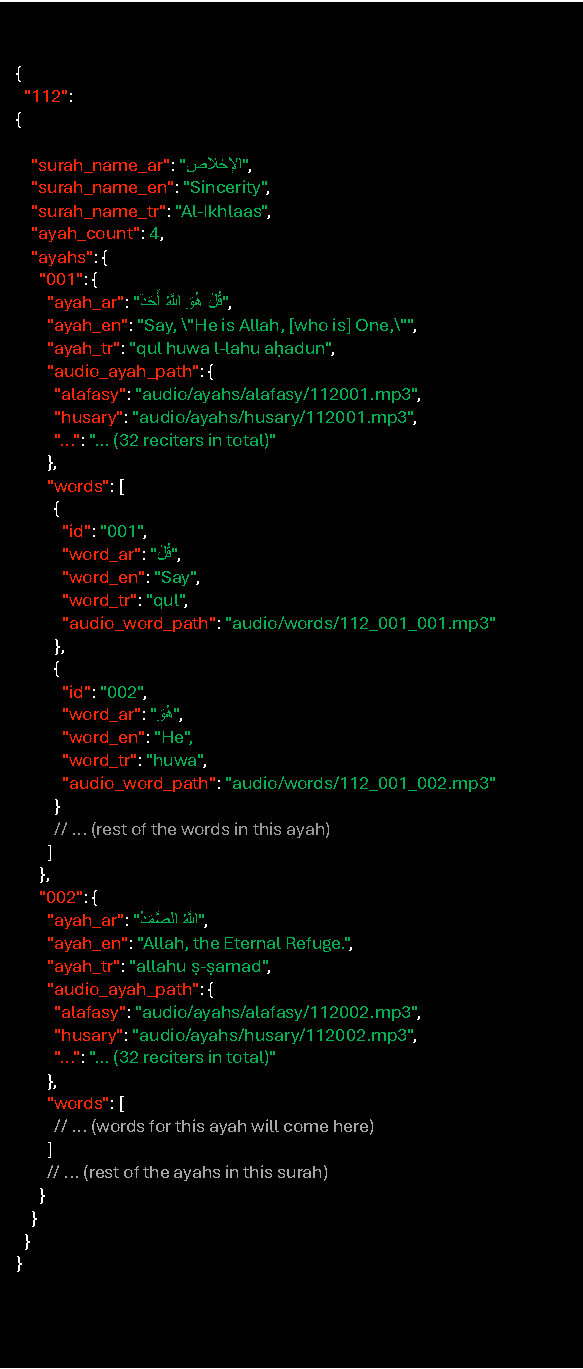
\includegraphics[width=0.31\textwidth]{figures/a.pdf} % Adjust width as needed
    \caption{Example of format of Surah 112 (Al-Ikhlas) in the Dataset.}
    \label{fig:example}
\end{figure}


\begin{table}[ht]
\centering
\caption{Overview of the \textsc{Qur’an-MD} dataset.}
\label{tab:dataset_stats}
\begin{tabular}{@{}lll@{}}
\toprule
\textbf{Category} & \textbf{Attribute} & \textbf{Statistics / Details} \\
\midrule
\multirow{3}{*}{Corpus Size} 
  & Surahs & 114 \\
  & Ayahs & 6,236 \\
  & Words & $\sim$77.8k \\
\addlinespace
\multirow{3}{*}{Audio} 
  & Reciters & 30 (diverse styles) \\
  & Verse-level Audio & $\sim$665 hours \\
  & Word-level Audio & $\sim$22 hours \\
\addlinespace
\multirow{2}{*}{Modalities} 
  & Text & Arabic, English, Transliteration \\
  & Audio & Verse- and Word-level recordings \\
\bottomrule
\end{tabular}
\end{table}








\bibliographystyle{unsrt}
\bibliography{references}

% \newpage
% \section*{NeurIPS Paper Checklist}

% \begin{enumerate}

% \item {\bf Claims}
%     \item[] Question: Do the main claims made in the abstract and introduction accurately reflect the paper's contributions and scope?
%     \item[] Answer: \answerYes{} % Replace by \answerYes{}, \answerNo{}, or \answerNA{}.
%     \item[] Justification: The abstract and introduction clearly describe the paper’s primary contribution: the construction of a multimodal Qur’an dataset that integrates text, translation, transliteration, and aligned audio across multiple speakers at both the verse and word levels. The claims are descriptive rather than exaggerated, and they align with what the dataset actually provides. The scope is well defined as a resource paper, with potential applications (e.g., ASR, TTS, NLP, and tajweed analysis) mentioned as opportunities for future work rather than as current achievements. This ensures that the abstract and introduction accurately reflect the contributions without overstating results or generalization.
%     \item[] Guidelines:
%     \begin{itemize}
%         \item The answer NA means that the abstract and introduction do not include the claims made in the paper.
%         \item The abstract and/or introduction should clearly state the claims made, including the contributions made in the paper and important assumptions and limitations. A No or NA answer to this question will not be perceived well by the reviewers. 
%         \item The claims made should match theoretical and experimental results, and reflect how much the results can be expected to generalize to other settings. 
%         \item It is fine to include aspirational goals as motivation as long as it is clear that these goals are not attained by the paper. 
%     \end{itemize}

% \item {\bf Limitations}
%     \item[] Question: Does the paper discuss the limitations of the work performed by the authors?
%     \item[] Answer: \answerNA{} % Replace by \answerYes{}, \answerNo{}, or \answerNA{}.
%     \item[] Justification: The paper does not explicitly include a discussion of limitations. While some scope boundaries can be inferred from the description of the dataset, a dedicated limitations section is not provided. As such, the work is presented without a clear reflection on assumptions, potential shortcomings, or constraints.
%     \item[] Guidelines:
%     \begin{itemize}
%         \item The answer NA means that the paper has no limitation while the answer No means that the paper has limitations, but those are not discussed in the paper. 
%         \item The authors are encouraged to create a separate "Limitations" section in their paper.
%         \item The paper should point out any strong assumptions and how robust the results are to violations of these assumptions (e.g., independence assumptions, noiseless settings, model well-specification, asymptotic approximations only holding locally). The authors should reflect on how these assumptions might be violated in practice and what the implications would be.
%         \item The authors should reflect on the scope of the claims made, e.g., if the approach was only tested on a few datasets or with a few runs. In general, empirical results often depend on implicit assumptions, which should be articulated.
%         \item The authors should reflect on the factors that influence the performance of the approach. For example, a facial recognition algorithm may perform poorly when image resolution is low or images are taken in low lighting. Or a speech-to-text system might not be used reliably to provide closed captions for online lectures because it fails to handle technical jargon.
%         \item The authors should discuss the computational efficiency of the proposed algorithms and how they scale with dataset size.
%         \item If applicable, the authors should discuss possible limitations of their approach to address problems of privacy and fairness.
%         \item While the authors might fear that complete honesty about limitations might be used by reviewers as grounds for rejection, a worse outcome might be that reviewers discover limitations that aren't acknowledged in the paper. The authors should use their best judgment and recognize that individual actions in favor of transparency play an important role in developing norms that preserve the integrity of the community. Reviewers will be specifically instructed to not penalize honesty concerning limitations.
%     \end{itemize}

% \item {\bf Theory assumptions and proofs}
%     \item[] Question: For each theoretical result, does the paper provide the full set of assumptions and a complete (and correct) proof?
%     \item[] Answer: \answerNA{}% Replace by \answerYes{}, \answerNo{}, or \answerNA{}.
%     \item[] Justification: The paper's contribution is the creation and description of a new dataset. It does not introduce any theoretical results, theorems, or mathematical proofs that would require such justification.
%     \item[] Guidelines:
%     \begin{itemize}
%         \item The answer NA means that the paper does not include theoretical results. 
%         \item All the theorems, formulas, and proofs in the paper should be numbered and cross-referenced.
%         \item All assumptions should be clearly stated or referenced in the statement of any theorems.
%         \item The proofs can either appear in the main paper or the supplemental material, but if they appear in the supplemental material, the authors are encouraged to provide a short proof sketch to provide intuition. 
%         \item Inversely, any informal proof provided in the core of the paper should be complemented by formal proofs provided in appendix or supplemental material.
%         \item Theorems and Lemmas that the proof relies upon should be properly referenced. 
%     \end{itemize}

%     \item {\bf Experimental result reproducibility}
%     \item[] Question: Does the paper fully disclose all the information needed to reproduce the main experimental results of the paper to the extent that it affects the main claims and/or conclusions of the paper (regardless of whether the code and data are provided or not)?
%     \item[] Answer: \answerYes{} % Replace by \answerYes{}, \answerNo{}, or \answerNA{}.
%     \item[] Justification: The paper's main contribution is a dataset, not experimental results in a traditional sense. It clearly discloses the methodology for the dataset's creation by identifying the three public sources used and detailing the four-step pipeline for data aggregation, harmonization, and validation. This is sufficient to understand how the dataset was constructed.
%     \item[] Guidelines:
%     \begin{itemize}
%         \item The answer NA means that the paper does not include experiments.
%         \item If the paper includes experiments, a No answer to this question will not be perceived well by the reviewers: Making the paper reproducible is important, regardless of whether the code and data are provided or not.
%         \item If the contribution is a dataset and/or model, the authors should describe the steps taken to make their results reproducible or verifiable. 
%         \item Depending on the contribution, reproducibility can be accomplished in various ways. For example, if the contribution is a novel architecture, describing the architecture fully might suffice, or if the contribution is a specific model and empirical evaluation, it may be necessary to either make it possible for others to replicate the model with the same dataset, or provide access to the model. In general. releasing code and data is often one good way to accomplish this, but reproducibility can also be provided via detailed instructions for how to replicate the results, access to a hosted model (e.g., in the case of a large language model), releasing of a model checkpoint, or other means that are appropriate to the research performed.
%         \item While NeurIPS does not require releasing code, the conference does require all submissions to provide some reasonable avenue for reproducibility, which may depend on the nature of the contribution. For example
%         \begin{enumerate}
%             \item If the contribution is primarily a new algorithm, the paper should make it clear how to reproduce that algorithm.
%             \item If the contribution is primarily a new model architecture, the paper should describe the architecture clearly and fully.
%             \item If the contribution is a new model (e.g., a large language model), then there should either be a way to access this model for reproducing the results or a way to reproduce the model (e.g., with an open-source dataset or instructions for how to construct the dataset).
%             \item We recognize that reproducibility may be tricky in some cases, in which case authors are welcome to describe the particular way they provide for reproducibility. In the case of closed-source models, it may be that access to the model is limited in some way (e.g., to registered users), but it should be possible for other researchers to have some path to reproducing or verifying the results.
%         \end{enumerate}
%     \end{itemize}


% \item {\bf Open access to data and code}
%     \item[] Question: Does the paper provide open access to the data and code, with sufficient instructions to faithfully reproduce the main experimental results, as described in supplemental material?
%     \item[] Answer: \answerYes{}{} % Replace by \answerYes{}, \answerNo{}, or \answerNA{}.
%     \item[] Justification: The paper explicitly states that "The dataset curation code will be released, and the dataset itself will be made publicly available". It further specifies that the dataset will be released on Hugging Face, a standard platform for sharing research assets, ensuring community access.
%     \item[] Guidelines:
%     \begin{itemize}
%         \item The answer NA means that paper does not include experiments requiring code.
%         \item Please see the NeurIPS code and data submission guidelines (\url{https://nips.cc/public/guides/CodeSubmissionPolicy}) for more details.
%         \item While we encourage the release of code and data, we understand that this might not be possible, so “No” is an acceptable answer. Papers cannot be rejected simply for not including code, unless this is central to the contribution (e.g., for a new open-source benchmark).
%         \item The instructions should contain the exact command and environment needed to run to reproduce the results. See the NeurIPS code and data submission guidelines (\url{https://nips.cc/public/guides/CodeSubmissionPolicy}) for more details.
%         \item The authors should provide instructions on data access and preparation, including how to access the raw data, preprocessed data, intermediate data, and generated data, etc.
%         \item The authors should provide scripts to reproduce all experimental results for the new proposed method and baselines. If only a subset of experiments are reproducible, they should state which ones are omitted from the script and why.
%         \item At submission time, to preserve anonymity, the authors should release anonymized versions (if applicable).
%         \item Providing as much information as possible in supplemental material (appended to the paper) is recommended, but including URLs to data and code is permitted.
%     \end{itemize}


% \item {\bf Experimental setting/details}
%     \item[] Question: Does the paper specify all the training and test details (e.g., data splits, hyperparameters, how they were chosen, type of optimizer, etc.) necessary to understand the results?
%     \item[] Answer: \answerNA{} % Replace by \answerYes{}, \answerNo{}, or \answerNA{}.
%     \item[] Justification: The paper does not conduct experiments that involve model training or evaluation. Its focus is on the curation of a dataset, so details regarding experimental settings like hyperparameters or data splits are not applicable.
%     \item[] Guidelines:
%     \begin{itemize}
%         \item The answer NA means that the paper does not include experiments.
%         \item The experimental setting should be presented in the core of the paper to a level of detail that is necessary to appreciate the results and make sense of them.
%         \item The full details can be provided either with the code, in appendix, or as supplemental material.
%     \end{itemize}

% \item {\bf Experiment statistical significance}
%     \item[] Question: Does the paper report error bars suitably and correctly defined or other appropriate information about the statistical significance of the experiments?
%     \item[] Answer: \answerNA{} % Replace by \answerYes{}, \answerNo{}, or \answerNA{}.
%     \item[] Justification: This is a resource paper that describes a dataset. It does not report quantitative experimental results that would require statistical significance testing or error bars.
%     \item[] Guidelines:
%     \begin{itemize}
%         \item The answer NA means that the paper does not include experiments.
%         \item The authors should answer "Yes" if the results are accompanied by error bars, confidence intervals, or statistical significance tests, at least for the experiments that support the main claims of the paper.
%         \item The factors of variability that the error bars are capturing should be clearly stated (for example, train/test split, initialization, random drawing of some parameter, or overall run with given experimental conditions).
%         \item The method for calculating the error bars should be explained (closed form formula, call to a library function, bootstrap, etc.)
%         \item The assumptions made should be given (e.g., Normally distributed errors).
%         \item It should be clear whether the error bar is the standard deviation or the standard error of the mean.
%         \item It is OK to report 1-sigma error bars, but one should state it. The authors should preferably report a 2-sigma error bar than state that they have a 96\% CI, if the hypothesis of Normality of errors is not verified.
%         \item For asymmetric distributions, the authors should be careful not to show in tables or figures symmetric error bars that would yield results that are out of range (e.g. negative error rates).
%         \item If error bars are reported in tables or plots, The authors should explain in the text how they were calculated and reference the corresponding figures or tables in the text.
%     \end{itemize}

% \item {\bf Experiments compute resources}
%     \item[] Question: For each experiment, does the paper provide sufficient information on the computer resources (type of compute workers, memory, time of execution) needed to reproduce the experiments?
%     \item[] Answer: \answerNA{} % Replace by \answerYes{}, \answerNo{}, or \answerNA{}.
%     \item[] Justification: The paper's contribution is a dataset and does not involve computational experiments like model training. Therefore, information about compute resources is not applicable.
%     \item[] Guidelines:
%     \begin{itemize}
%         \item The answer NA means that the paper does not include experiments.
%         \item The paper should indicate the type of compute workers CPU or GPU, internal cluster, or cloud provider, including relevant memory and storage.
%         \item The paper should provide the amount of compute required for each of the individual experimental runs as well as estimate the total compute. 
%         \item The paper should disclose whether the full research project required more compute than the experiments reported in the paper (e.g., preliminary or failed experiments that didn't make it into the paper). 
%     \end{itemize}
    
% \item {\bf Code of ethics}
%     \item[] Question: Does the research conducted in the paper conform, in every respect, with the NeurIPS Code of Ethics \url{https://neurips.cc/public/EthicsGuidelines}?
%     \item[] Answer: \answerYes{}{} % Replace by \answerYes{}, \answerNo{}, or \answerNA{}.
%     \item[] Justification: The research involves the curation of publicly available data to create a resource for academic and community use. The work is handled with respect for the cultural and religious significance of the source material (the Quran) and aims to provide a tool for educational and research advancement, aligning with ethical guidelines.
%     \item[] Guidelines:
%     \begin{itemize}
%         \item The answer NA means that the authors have not reviewed the NeurIPS Code of Ethics.
%         \item If the authors answer No, they should explain the special circumstances that require a deviation from the Code of Ethics.
%         \item The authors should make sure to preserve anonymity (e.g., if there is a special consideration due to laws or regulations in their jurisdiction).
%     \end{itemize}


% \item {\bf Broader impacts}
%     \item[] Question: Does the paper discuss both potential positive societal impacts and negative societal impacts of the work performed?
%     \item[] Answer: \answerYes{}{} % Replace by \answerYes{}, \answerNo{}, or \answerNA{}.
%     \item[] Justification: The paper extensively discusses positive societal impacts, such as developing educational tools for recitation , supporting linguistic analysis, and fostering broader community engagement with Quranic studies. While it does not explicitly detail negative impacts, the work, a structured dataset of a public religious text, does not present obvious direct paths to misuse.
%     \item[] Guidelines:
%     \begin{itemize}
%         \item The answer NA means that there is no societal impact of the work performed.
%         \item If the authors answer NA or No, they should explain why their work has no societal impact or why the paper does not address societal impact.
%         \item Examples of negative societal impacts include potential malicious or unintended uses (e.g., disinformation, generating fake profiles, surveillance), fairness considerations (e.g., deployment of technologies that could make decisions that unfairly impact specific groups), privacy considerations, and security considerations.
%         \item The conference expects that many papers will be foundational research and not tied to particular applications, let alone deployments. However, if there is a direct path to any negative applications, the authors should point it out. For example, it is legitimate to point out that an improvement in the quality of generative models could be used to generate deepfakes for disinformation. On the other hand, it is not needed to point out that a generic algorithm for optimizing neural networks could enable people to train models that generate Deepfakes faster.
%         \item The authors should consider possible harms that could arise when the technology is being used as intended and functioning correctly, harms that could arise when the technology is being used as intended but gives incorrect results, and harms following from (intentional or unintentional) misuse of the technology.
%         \item If there are negative societal impacts, the authors could also discuss possible mitigation strategies (e.g., gated release of models, providing defenses in addition to attacks, mechanisms for monitoring misuse, mechanisms to monitor how a system learns from feedback over time, improving the efficiency and accessibility of ML).
%     \end{itemize}
    
% \item {\bf Safeguards}
%     \item[] Question: Does the paper describe safeguards that have been put in place for responsible release of data or models that have a high risk for misuse (e.g., pretrained language models, image generators, or scraped datasets)?
%     \item[] Answer: \answerNA{}{} % Replace by \answerYes{}, \answerNo{}, or \answerNA{}.
%     \item[] Justification: The dataset is compiled from publicly available sources of a religious text and its recitation. It does not contain sensitive personal information or generative models with a high potential for misuse, so special safeguards are not applicable.
%     \item[] Guidelines:
%     \begin{itemize}
%         \item The answer NA means that the paper poses no such risks.
%         \item Released models that have a high risk for misuse or dual-use should be released with necessary safeguards to allow for controlled use of the model, for example by requiring that users adhere to usage guidelines or restrictions to access the model or implementing safety filters. 
%         \item Datasets that have been scraped from the Internet could pose safety risks. The authors should describe how they avoided releasing unsafe images.
%         \item We recognize that providing effective safeguards is challenging, and many papers do not require this, but we encourage authors to take this into account and make a best faith effort.
%     \end{itemize}

% \item {\bf Licenses for existing assets}
%     \item[] Question: Are the creators or original owners of assets (e.g., code, data, models), used in the paper, properly credited and are the license and terms of use explicitly mentioned and properly respected?
%     \item[] Answer: \answerYes{}{} % Replace by \answerYes{}, \answerNo{}, or \answerNA{}.
%     \item[] Justification: The paper properly credits the original owners of the three source datasets by citing them directly and providing URLs in the references. This allows users to access the original assets and view their respective licenses and terms of use.
%     \item[] Guidelines:
%     \begin{itemize}
%         \item The answer NA means that the paper does not use existing assets.
%         \item The authors should cite the original paper that produced the code package or dataset.
%         \item The authors should state which version of the asset is used and, if possible, include a URL.
%         \item The name of the license (e.g., CC-BY 4.0) should be included for each asset.
%         \item For scraped data from a particular source (e.g., website), the copyright and terms of service of that source should be provided.
%         \item If assets are released, the license, copyright information, and terms of use in the package should be provided. For popular datasets, \url{paperswithcode.com/datasets} has curated licenses for some datasets. Their licensing guide can help determine the license of a dataset.
%         \item For existing datasets that are re-packaged, both the original license and the license of the derived asset (if it has changed) should be provided.
%         \item If this information is not available online, the authors are encouraged to reach out to the asset's creators.
%     \end{itemize}

% \item {\bf New assets}
%     \item[] Question: Are new assets introduced in the paper well documented and is the documentation provided alongside the assets?
%     \item[] Answer: \answerYes{}{} % Replace by \answerYes{}, \answerNo{}, or \answerNA{}.
%     \item[] Justification: The new asset, the Quran-MD dataset, is well-documented within the paper. The methodology for its creation is described in Section 3 , its hierarchical JSON structure is detailed in Section 4 , and a clear example is provided in the appendix.
%     \item[] Guidelines:
%     \begin{itemize}
%         \item The answer NA means that the paper does not release new assets.
%         \item Researchers should communicate the details of the dataset/code/model as part of their submissions via structured templates. This includes details about training, license, limitations, etc. 
%         \item The paper should discuss whether and how consent was obtained from people whose asset is used.
%         \item At submission time, remember to anonymize your assets (if applicable). You can either create an anonymized URL or include an anonymized zip file.
%     \end{itemize}

% \item {\bf Crowdsourcing and research with human subjects}
%     \item[] Question: For crowdsourcing experiments and research with human subjects, does the paper include the full text of instructions given to participants and screenshots, if applicable, as well as details about compensation (if any)? 
%     \item[] Answer: \answerNA{} % Replace by \answerYes{}, \answerNo{}, or \answerNA{}.
%     \item[] Justification: The paper does not involve any new crowdsourcing or direct research with human subjects. It curates the dataset from existing public sources.
%     \item[] Guidelines:
%     \begin{itemize}
%         \item The answer NA means that the paper does not involve crowdsourcing nor research with human subjects.
%         \item Including this information in the supplemental material is fine, but if the main contribution of the paper involves human subjects, then as much detail as possible should be included in the main paper. 
%         \item According to the NeurIPS Code of Ethics, workers involved in data collection, curation, or other labor should be paid at least the minimum wage in the country of the data collector. 
%     \end{itemize}

% \item {\bf Institutional review board (IRB) approvals or equivalent for research with human subjects}
%     \item[] Question: Does the paper describe potential risks incurred by study participants, whether such risks were disclosed to the subjects, and whether Institutional Review Board (IRB) approvals (or an equivalent approval/review based on the requirements of your country or institution) were obtained?
%     \item[] Answer: \answerNA{}{} % Replace by \answerYes{}, \answerNo{}, or \answerNA{}.
%     \item[] Justification: As the research did not involve new experiments with human subjects, IRB approval was not applicable.
%     \item[] Guidelines:
%     \begin{itemize}
%         \item The answer NA means that the paper does not involve crowdsourcing nor research with human subjects.
%         \item Depending on the country in which research is conducted, IRB approval (or equivalent) may be required for any human subjects research. If you obtained IRB approval, you should clearly state this in the paper. 
%         \item We recognize that the procedures for this may vary significantly between institutions and locations, and we expect authors to adhere to the NeurIPS Code of Ethics and the guidelines for their institution. 
%         \item For initial submissions, do not include any information that would break anonymity (if applicable), such as the institution conducting the review.
%     \end{itemize}

% \item {\bf Declaration of LLM usage}
%     \item[] Question: Does the paper describe the usage of LLMs if it is an important, original, or non-standard component of the core methods in this research? Note that if the LLM is used only for writing, editing, or formatting purposes and does not impact the core methodology, scientific rigorousness, or originality of the research, declaration is not required.
%     %this research? 
%     \item[] Answer: \answerNA{}{} % Replace by \answerYes{}, \answerNo{}, or \answerNA{}.
%     \item[] Justification: The core methodology involved data aggregation, alignment, and structuring from existing public sources. LLMs were not a component of the dataset curation process.
%     \item[] Guidelines:
%     \begin{itemize}
%         \item The answer NA means that the core method development in this research does not involve LLMs as any important, original, or non-standard components.
%         \item Please refer to our LLM policy (\url{https://neurips.cc/Conferences/2025/LLM}) for what should or should not be described.
%     \end{itemize}

% \end{enumerate}


\end{document}